\documentclass[a4paper, 11pt]{article}         % Paper and font size
\usepackage[english]{babel}                     % Language setting
% \usepackage[style=authoryear-ibid,backend=biber]{biblatex}
\usepackage[style=numeric,backend=biber]{biblatex}
\addbibresource{bibliography.bib}

% Customize your title, name, place and date here to change title, header, footer, etc.
\newcommand{\titlefirstpage}{A direct summation 3d simulation of a globular cluster}
\newcommand{\titleheaderline}{\titlefirstpage{}}
\newcommand{\authorname}{Leonardo Quiñonez}
\newcommand{\authormail}{a12411091@unet.univie.ac.at}
\newcommand{\authordate}{\today{}}
\newcommand{\authorplace}{Wien}

% Set margins
\usepackage[top=2.5cm,bottom=2.5cm,left=2cm,right=2cm,marginparwidth=1.75cm]{geometry}

% Load useful packages
\usepackage{graphicx}                           % Graphics
\usepackage{amsmath}                            % Math
\usepackage{xcolor}                             % Link color
\usepackage{subcaption}
\definecolor{custom-blue}{RGB}{0,99,166} 
\usepackage{hyperref}
\hypersetup{colorlinks=true, allcolors=custom-blue}

\usepackage{fancyhdr}                           % Load header, footer package
\usepackage{csquotes}                           % textcite, parencite, etc.
\usepackage{lastpage}                           % Footer note
\usepackage{lipsum}                             % For dummy text
\usepackage[                                    % \say for quotation marks
                                                % configure to use german-style quotes
left = \glqq,%
right = \grqq,%
leftsub = \glq,%
rightsub = \grq%
]{dirtytalk}

\pagestyle{myheadings}                          % Own header
\pagestyle{fancy}                               % Own style
\fancyhf{}                                      % Clear header, footer

\setlength{\headheight}{30pt}                   % Set header hight
\renewcommand{\headrulewidth}{0.5pt}            % Top line
\renewcommand{\footrulewidth}{0.5pt}            % Bottom line

\fancyhead[L]{
\includegraphics[width=3cm]{univienna-logo.eps}} % Header left
\fancyhead[C]{}                                                % Header center
\fancyhead[R]{\titleheaderline}                                % Header right
\fancyfoot[L]{\authorname}                                     % Footer left
\fancyfoot[C]{                                                 % Footer center
  \thepage
  % uncomment next line also include the total page count
  % /\pageref{LastPage}
}
\fancyfoot[R]{test}                                   % Footer right

%%% Begin document %%%
\begin{document}

\begin{figure}                                  % Include Logo
\flushleft

\includegraphics[width=0.4\textwidth]{univienna-logo.eps}
\end{figure}

% Set title, author, date
\title{\titlefirstpage{} \\ \large Focus project for Methods of Computational Astrophysics}

\author{\authorname{} - \authormail{}}
\date{\authordate, \authorplace}

\maketitle                                      % Include contents
%\tableofcontents

\section{Problem}                              % Example sections, subsections

The N-body problem is a great test bed for computational methods,
multiple different techniques have been developed to tackle it, some of which were explored during the course. \parencite{Hahn2025classnotes}

The goal of this focus project is to do a 3D particle simulation  of a globular cluster, using the direct summation method. 
The objective is to set the positions and velocities following a Plummer Model for the globular cluster. Then using a leapfrog integrator evolve the system in time. The integrator calls an acceleration function which we try to make as performant as possible. Finally, a video of the simulation closes the project.

The main focus of the project is on finding an efficient implementation for the direct summation,
since it is the most computationally heavy part with a complexity of \( \mathcal{O}(N^2) \) for \( N \) particles. The different worksheets done during the class are good stepping stones for this.



\section{Approach}                              % Example sections, subsections
The project was subdivided in the following steps:
\begin{enumerate}
    \item Efficient Direct Summation
    \item Time Integration
    \item 3D Simulation
    \item Initial Conditions
\end{enumerate}


\paragraph{Efficient Direct Summation:}
We start working on the direct summation, taking the work done on worksheet 1.
To do the simulation with dimensionless units and equal masses we define the acceleration for particle $X_i$ as:

\begin{subequations}
\begin{align}
    a(X_i) &= -\sum_{\substack{j=1 \\ j \ne i}}^{N} \frac{\mathbf{X}_i - \mathbf{X}_j}{\|\mathbf{X}_i - \mathbf{X}_j\|^3} \label{eq:motion_b}
\end{align}
\end{subequations}

As suggested in worksheet 1 \parencite{ws1} we compare the computation speed of the different implementations.
The focus is on testing the limits of performance on large numbers of bodies. This is done scaling up exponentially the value of N until the computation time of the acceleration experienced by all the bodies  surpasses 10 seconds.

The implementations to test are:

\begin{itemize}
    \item Python loops
    \item Vectorized Numpy
    \item Numba (Loops)
    \item Numba (Parallel)
    \item Jax (CPU)
    \item Taichi (GPU --- added later)
\end{itemize}

Jax is only be tested on the CPU since the hardware available has no Nvidia GPU.

\paragraph{Time Integration:}
A leapfrog method is chosen for its simplicity but also energy conservation properties.
The Drift Kick Drift approach is selected to simplify the implementation and have only one acceleration calculation per time step.

\paragraph{3D simulation:}
A simple as possible 3D simulation is part of the objective, for this a search on possible libraries must be done.

\paragraph{Initial Conditions:}
Since we used the Plummer model during our worksheets its seems like a great starting point for our simulation. \parencite{ws5,ws7}



\section{Results}
The software written for the project can be found in Github at \url{https://github.com/laq/msc_comp-astro-proj} and the videos on the \href{https://drive.google.com/drive/folders/17HjF1KmQAJzP7fJ5GMh5vFHURGo9tkBM?usp=sharing}{shared drive}.


\subsection{Efficient Direct Summation}
\subsubsection{Taichi}
Originally the plan was to compare the implementations suggested in Worksheet 1\parencite{ws1} and incrementally do improvements on them. But, when searching for 3D animation libraries, we stumbled upon
Taichi Lang\footnote{Taichi Lang is a ``domain-specific language embedded in Python'' but for practical purposes it is installed like any other library. \parencite{TaichiLang}}. It allows the usage of Vulkan\parencite{Vulkan} to access the Intel integrated GPU for rendering and also computation.
Given that the available hardware possess no Nvidia GPU the original plan was expecting to limit computations to the CPU. However, an initial test with Taichi was so promising that it had to be included in the comparison even when not originally planned. Taichi can also be set to use the CPU, but setting up the test for both CPU and GPU was not trivial and the CPU results were unimpressive.

\subsubsection{Performance Comparison}

All tests were run on a laptop with 12th Gen Intel(R) Core(TM) i7-1250U and maximum performance selected, a max frequency of 4.7Ghz and 10 cores. The integrated GPU is an Alder Lake-UP4 GT2.
The available GPU only allows for 32 bit floats. To attempt a fair comparison between Jax and Taichi which seemed the fastest competitors we leave Jax on 32 bits as well. \footnote{Jax by default uses 32 bits but can be set for 64 bits with: \texttt{jax.config.update("jax\_enable\_x64", True) }}


In order to compare the performance of the different methods we increase the number of stars exponentially until the time to perform a single acceleration computation 
exceeds 10s. In order to account for compilation time of \texttt{jit} calls or other variations among runs, each implementation is run three times and the median is calculated.
During this process OOM(Out of Memory) errors started happening and hanging the machine.
This prompted to the addition of a memory usage limit of 1GB. 

The memory usage limit is accomplish by querying the operating system for the memory usage of the process ID every tenth of a second. This requires running each acceleration as a subprocess that can be killed if too much time or space is being used. Additionally, the memory usage calculation is far from exact.
But, even with this inaccuracy, the configuration was enough to avoid the OOM errors and see a full picture of all implementations performances in time and space.


Figures \ref{fig:time} \ref{fig:space} show the time and space comparisons. The space figure highlights the 3 implementations that have variations in space, leaving in gray the uneventful ones. 

The space graph shows the high memory usage of NumPy when reaching $10^4$ stars.
An inspection on the algorithm showed that the NumPy implementation which was an attempt to do a purely vectorized implementation has a fatal flaw. The pure vectorization is managed by calculating the distance of all bodies with each other in a single matrix, needing an NxN matrix. This means $10^4$ stars would need around 1.2Gbs of ram usage and $10^5$ would need 120Gbs.

Curiously enough Jax using \texttt{vmap} presents a similar memory issue.
It seems to be the case that, the current implementation requires as intermediate memory the vector of distances of the current star with all other stars, so a vector size N. Given that ``JAX might materialize the large intermediate matrix for all batch elements at once, requiring batch\_size * memory\_per\_intermediate\_matrix memory'' \parencite{JaxPerformance}, Jax presents a similar excessive memory usage pattern as NumPy.

An improved implementation with Jax's \texttt{lax.map} was additionally made, solving the memory issue.
This implementation using \texttt{lax.map} allows to set a batch size, the small tests on this increased progressively the memory usage without a visible impact on performance.


\begin{figure}
\centering
\begin{subfigure}{.5\textwidth}
  \centering
  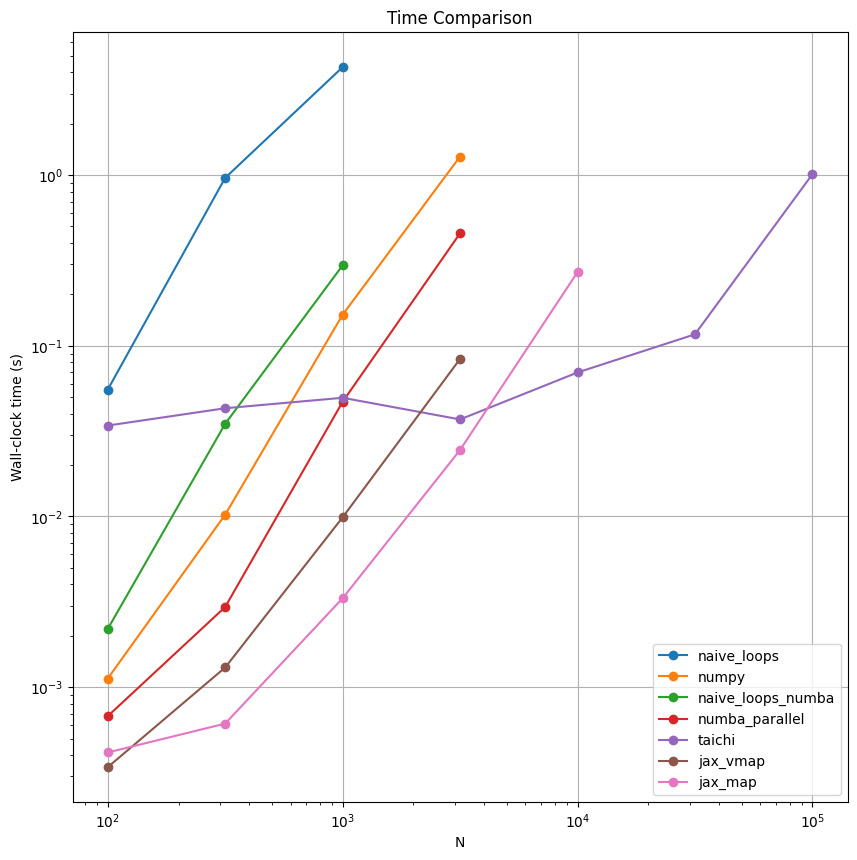
\includegraphics[width=\linewidth]{images/time_comp2}
  \caption{Time Comparison}
  \label{fig:time}
\end{subfigure}%
\begin{subfigure}{.5\textwidth}
  \centering
  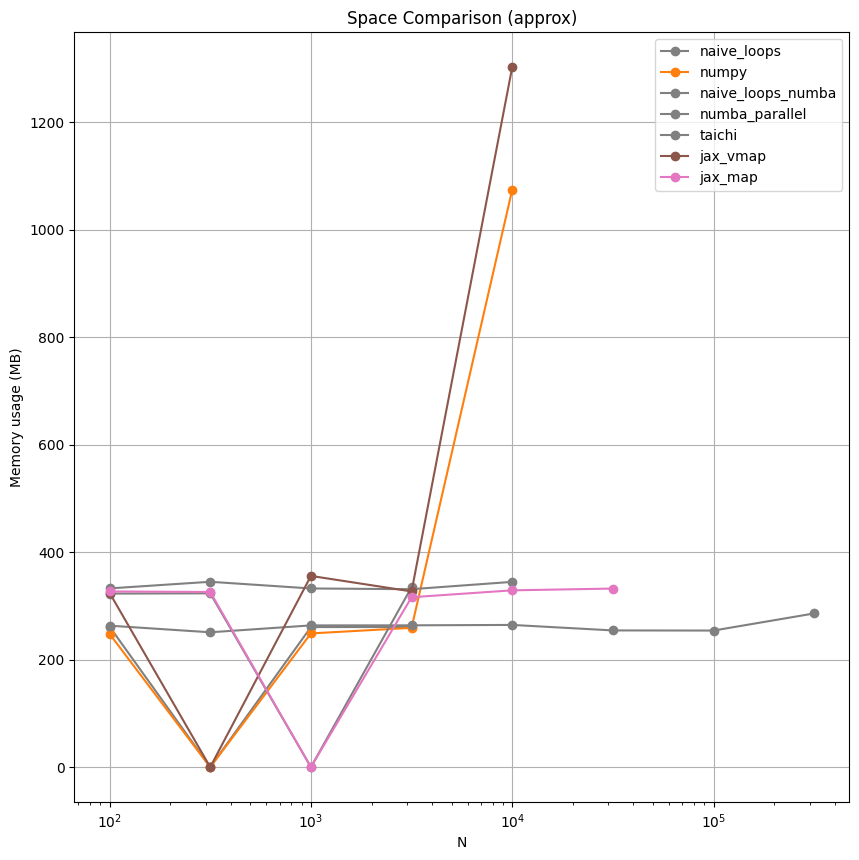
\includegraphics[width=\linewidth]{images/space_comp2}
  \caption{Space Comparison}
  \label{fig:space}
\end{subfigure}
\caption{Time and Space comparison capped to 10s and 1GB}
\label{fig:test}
\end{figure}

\subsection{Integration}
When testing with the Plummer model it became clear that a proper selection of the timesteps would be necessary
to keep stability and conserve energy, by the visual analysis on the simulation.
The best solution found was to scale the forces by a factor of $1/N$.

\subsection{3D simulation}
As mentioned earlier a search on options to simulate easily the cluster landed on Taichi. Its 3D rendering capacities are quite basic but also simple and powerful enough to use.
A basic proof of concept was easily done with the assistance of LLMS(Large Language Models). Iterating over this first proof of concept resulted in the current simulation.

The use of the local GPU for acceleration calculation and rendering allows simulating 40 thousand bodies at approximately 3.7 Frames per second, if additionally pictures are taken in every frame the performance reduces to around 2 Frames per second. Figures \ref{fig:plummer} and \ref{fig:multiple} show images of the resulting simulation. 

\begin{figure}
\centering
\begin{subfigure}{.5\textwidth}
  \centering
  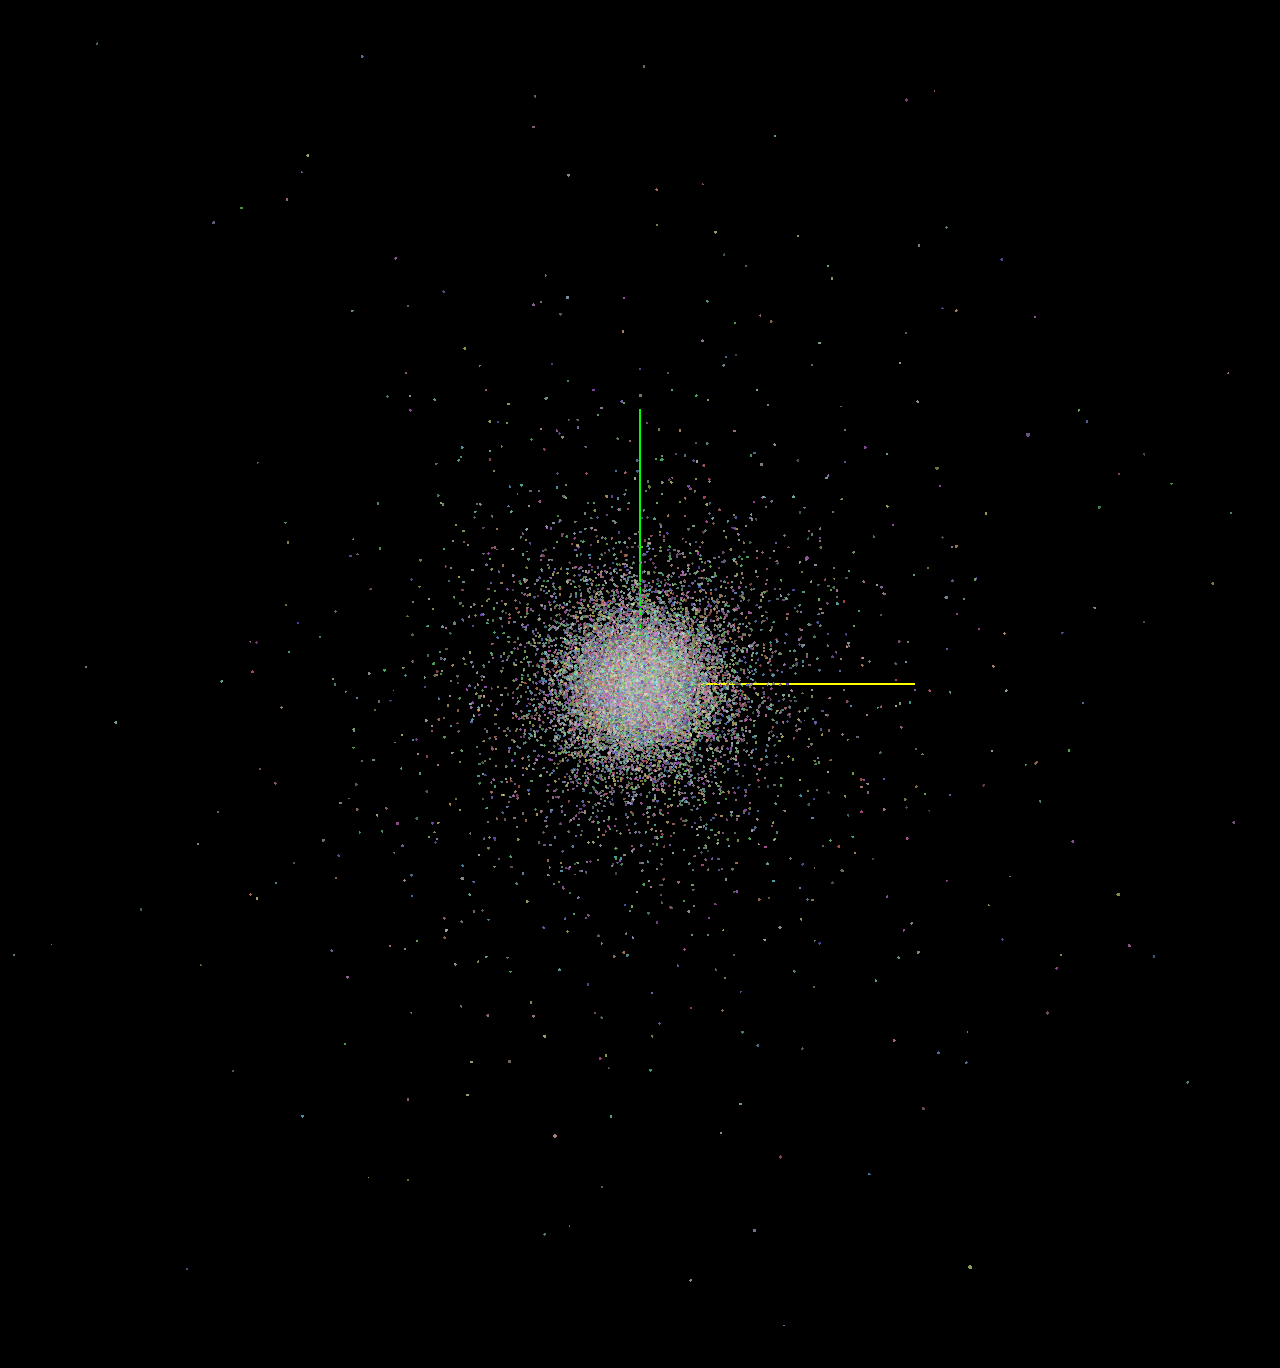
\includegraphics[clip, trim=6cm 6cm 6cm 6cm,width=\linewidth]{images/simulation}
  \caption{Plummer Model Simulation}
  \label{fig:plummer}
\end{subfigure}%
\begin{subfigure}{.5\textwidth}
  \centering
  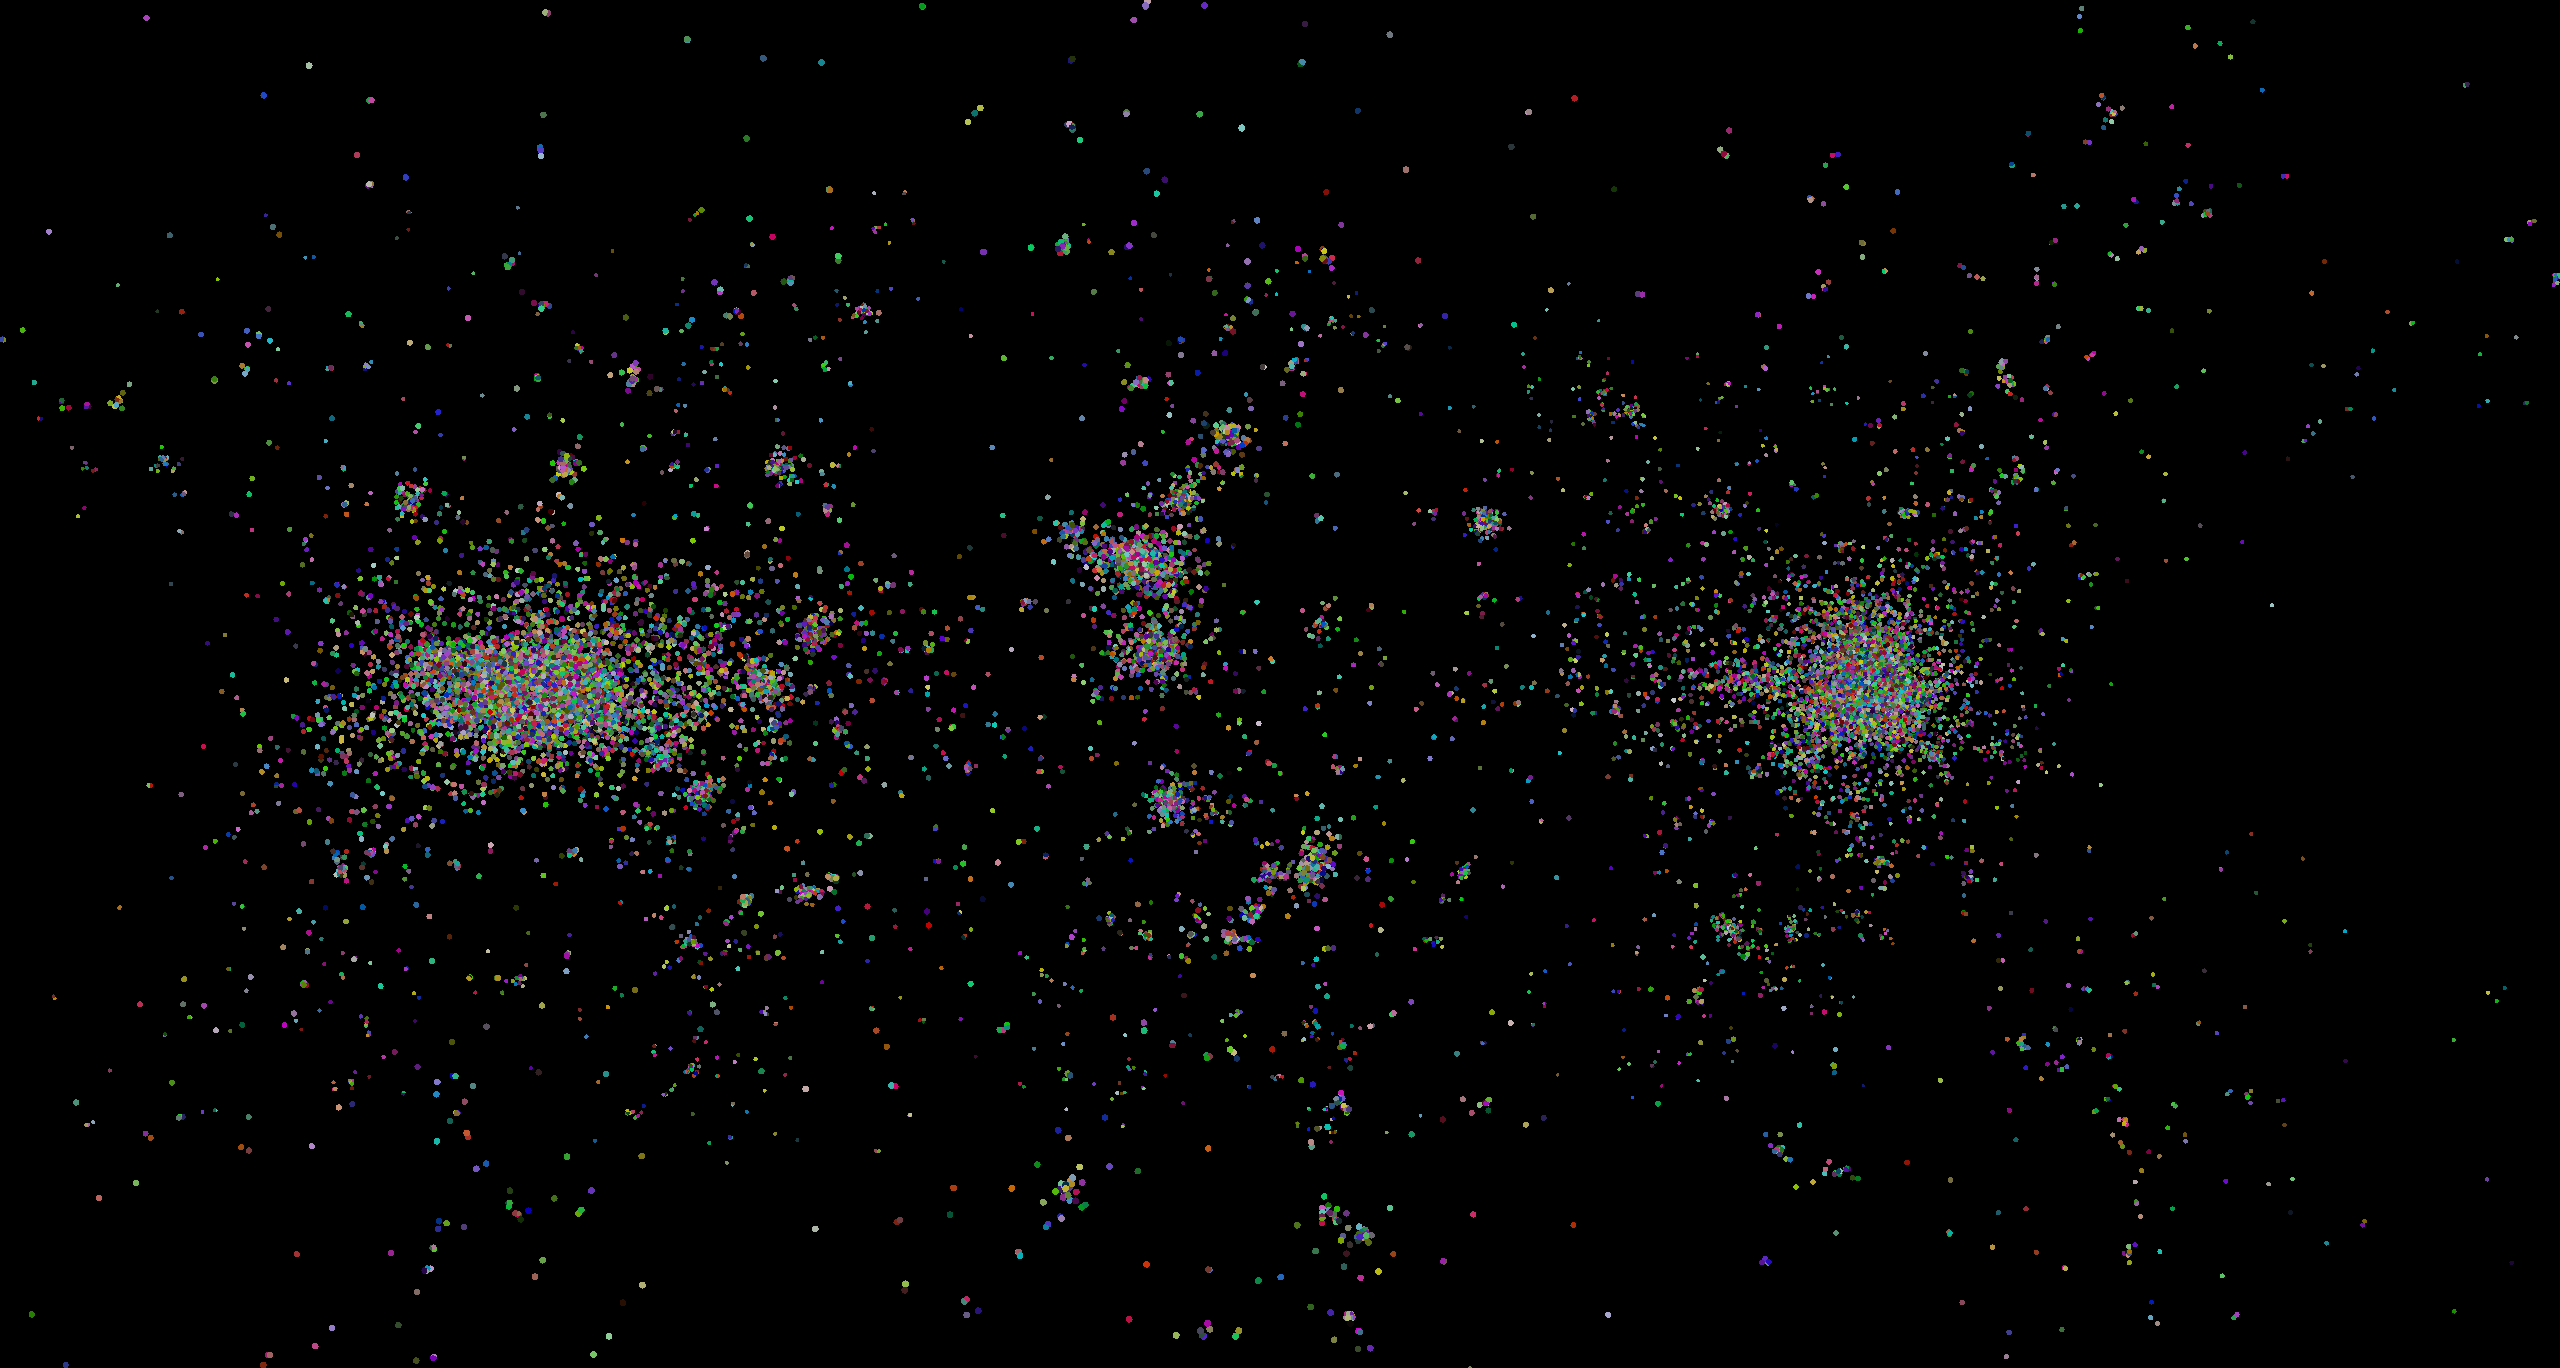
\includegraphics[clip, trim=6cm 0cm 6cm 0cm, width=\linewidth]{images/simulation2}
  \caption{Playing around with initial conditions}
  \label{fig:multiple}
\end{subfigure}
\caption{Frames from the simulation}
\label{fig:test}
\end{figure}

\section{Discussion}

\paragraph{Time Comparison:}
The comparison of the multiple algorithms showed that --- as expected --- using libraries that allow for parallelization and GPU usage greatly increases the number of particles that can be simulated. Most of the algorithms show the linear line that is expected on a log-log plot for the $O(N^2)$ algorithm. 
The exception being Taichi.
Stumbling upon Taichi, was a game changer. Its use of Vulkan enables the use of generic GPUs for the direct summation. Specifically it allowed to compute the acceleration on the integrated Intel Gpu available.
This allowed to compute an order of magnitude more of particles in comparison with Jax.\footnote{It is important to note that JAX can also use a GPU, but, to our knowledge, it is limited to Nvidia GPUs.}
Figure \ref{fig:time} shows this, but also shows how Taichi exhibits an almost flat behavior at smaller scales.
This could be due to the extra memory transfers required between GPU and CPU. However further testing would be necessary to understand this behavior.

Additionally, returning to Jax, the graph shows that Jax performs better when using \texttt{lax.map} compared to \texttt{jax.vmap}.

In summary, both Jax and Taichi had the best performance. However, given the constraints of the hardware, Taichi managed to calculate one order of magnitude more of stars.

\paragraph{Space Comparison:}
The space comparison became necessary when OOM errors first appeared.
These memory issues were quite interesting and unexpected. It was specially unexpected to encounter the issue with Jax, which lead to finding the documentation on vmap's drawbacks.

This made us realize that when simulating even larger numbers of stars additional problems will arise.
For example, the space necessary to hold all the positions and velocities or to store every position of every body in a file, in case one wants to split the integration and the rendering.


\paragraph{Rendering:}
The usage of Taichi provides a straightforward rendering mechanism with simple commands for camera movement.
Overall, the library is quite powerful, and LLMs are able to write simple proofs of concept without digging into the documentation. Unfortunately, when extending this code or doing specific tasks the LLMs get stuck and knowledge of the library becomes necessary. This might be an issue since documentation even when thorough was not always entirely clear. Probably doing the process in the right order and doing a Taichi tutorial to learn its basics would be properly rewarded when doing a full project using it.


\section{Future}
There are multiple directions this project could go forward.
The most natural followup is using more efficient algorithms for the force calculation, be it making use of the symmetries, implementing a hierarchical method or even using a spectral method.

For a hierarchical method probably a first implementation in NumPy would be useful as a stepping stone. Once its properly understood one could look onto porting it to Jax or Taichi. An interesting consideration is that hierarchical methods might change the number of bodies included in an acceleration calculation and Jax compiles each function separately for different sizes of the arguments.


It would be also interesting to test with an Nvidia gpu to compare Jax performance with Taichi on equal grounds.

Additionally, extra work on the integrator should be done. It would be interesting to plot the energy of the system and work towards ensuring stability and energy conservation.

\printbibliography[heading=bibintoc]

%%% End document %%%
\end{document}